\section{Compiler}\label{sec:compiler}

Damit eine Programmiersprache verwendbar ist, muss sie nicht nur eine Spezifikation haben, sondern auch ausführbar sein.
Dies kann durch direktes Ausführen des Programmtexts geschehen;
in diesem Fall wird das ausführende Programm Interpreter genannt.
Andererseits kann eine Programmiersprache auch in ein maschinenlesbares Format übersetzt werden,
das dann direkt oder durch eine virtuelle Maschine ausgeführt wird.
Dieser Ansatz nennt sich Kompilierung.
In Java wird die Kompilierung durch den Java Compiler (\code{javac}) durchgeführt, welcher Bytecode erzeugt;
dieser kann von einer Java Virtual Machine (JVM) ausgeführt werden.

FulibScenarios wird hingegen in zwei Schritten kompiliert.
Zunächst werden die Markdown-Scenario-Quelltexte in Java-Quelltexte übersetzt;
dies ist Aufgabe des Scenario-Compilers.
Der erzeugte Java-Quellcode wird dann vom Java-Compiler kompiliert.
Die Architektur und Implementierung des Scenario-Compilers sind Inhalt dieses Abschnitts.
Dabei wird des öfteren auf das Beispiel in Listing~\ref{lst:CompilationExample.md} Bezug genommen,
dessen Übersetzung bis zum Java-Quellcode in den einzelnen Teilabschnitten stückweise erarbeitet wird.

% TODO markdown
\codelisting{text}{chapter/fulib-scenarios/scenarios}{CompilationExample.md}{Beispiel-Szenario für diesen Abschnitt}

\subsection{Architektur}\label{subsec:compiler-architecture}

\todo{
Visitor Pattern~\cite{gof-design-patterns}.
Dragon Book~\cite{dragonbook}.
}

\begin{figure}
	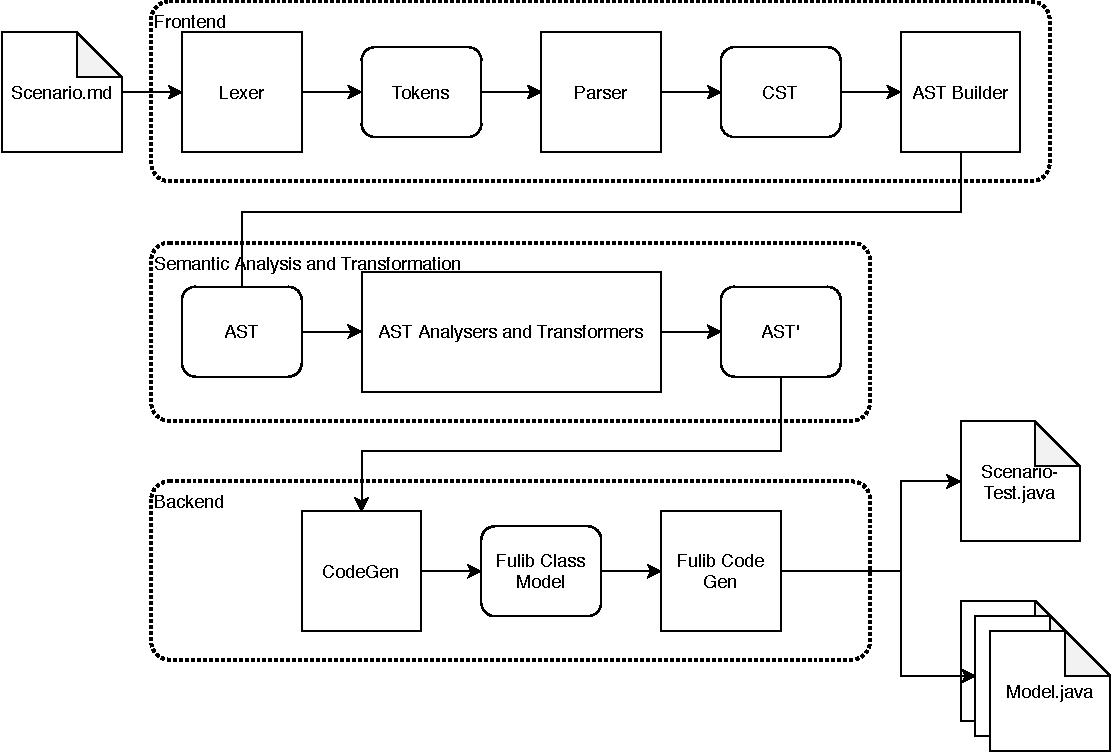
\includegraphics[width=\textwidth]{chapter/fulib-scenarios/img/architecture.pdf}
	\caption{Compiler-Architektur}
	\label{fig:compiler-architecture}
\end{figure}

\subsection{Frontend - ANTLR v4}\label{subsec:frontend-antlr4}

Die Übersetzung der Markdown-Datei beginnt mit deren Einlesen und Umwandeln in verarbeitbare Daten.
Im Compilerbau wird dies klassisch in zwei Phasen unterteilt:
Dem \emph{Lexer}, der die Zeichenfolge in eine Liste von Wörtern mit Typinformationen, genannt \emph{Tokens}, umwandelt;
und dem \emph{Parser}, der die flache Liste von Tokens nach den Regeln der Grammatik in eine Baumstruktur bringt,
die \emph{Concrete Syntax Tree (CST)} genannt wird.

Da die Umwandlung in Tokens und deren Strukturierung Anwendung in den meisten Compilern findet
und deren Implementierung meist nach einem festen Muster stattfindet,
existieren Tools, die diesen Prozess vereinfachen.
Diese werden \emph{Compiler-Compiler} oder \emph{Lexer- und Parsergeneratoren} genannt.

Das Frontend des Scenario-Compilers basiert auf dem Parsergenerator ANTLR4~\cite{antlr4-reference}.
Mit diesem können Grammatiken in einem EBNF-ähnlichen Format spezifiziert werden.
Aus der Grammatik generiert das Tool dann Java-Code, der Dateien einlesen kann und einen CST generiert.

Zunächst soll betrachtet werden, wie die FulibScenarios-Grammatik definiert ist.
Dies beginnt mit der Definition des Lexers.
In Listing~\ref{lst:ScenarioLexer.g4} ist ein Ausschnitt der ANTLR4-Grammatik zu sehen, die diesen definiert.
Der Ausschnitt ist ausreichend um das Scenario aus Listing~\ref{lst:CompilationExample.md} verarbeiten zu können;
die eigentliche Grammatik von FulibScenarios besteht aus vielen weiteren Regeln, um alle Funktionen der Sprache zu implementieren.
Sie ist in Anhang~\ref{sec:scenario-lexer-grammar} zu finden.

\codelisting{antlr}{chapter/fulib-scenarios/grammars}{ScenarioLexer.g4}{Ausschnitt der Scenario-Lexer-Grammatik}

Die Grammatik besteht aus mehreren Regeln, die einem Muster einen Namen zuordnen.
Dieser Name wird später den Tokens zugeordnet.
So haben Tokens mit dem Text \code{and} später den Namen \code{AND};
und jene, die eine Zahl darstellen, den Namen \code{INTEGER}.
Im Folgenden werden Tokens mit der Kurzschreibweise \code{<name>(<text>)} bezeichnet,
z.B.\ \code{AND(and)} und \code{INTEGER(12)}.

Die rechte Seite jeder Regel ähnelt einem regulären Ausdruck.
Bei Schlüsselwörtern wie \code{a}, \code{is} und \code{with} muss der Text exakt entsprechen;
\code{There} darf beispielsweise auch kleingeschrieben werden.
Ein \code{HEADLINE}-Token entsteht, wenn auf ein \code{#}-Zeichen beliebig viele Zeichen und ein Zeilenumbruch folgen\footnote{
Dabei bedeutet \code{~[\n]*?} \outquote{beliebig viele Zeichen ausgenommen Zeilenumbruch}.}.
Ganze Zahlen können mit einem Minus-Zeichen beginnen und bestehen aus mindestens einer Ziffer.
Wörter beginnen mit einem Buchstaben, gefolgt von beliebig vielen Buchstaben, Ziffern, Apostrophen, Unterstrichen und Bindestrichen.
Die Regel \code{WS} sorgt durch die Angabe \code{-> skip} dafür, dass keine Whitespace-Zeichen zu Token werden.
Falls mehrere Regeln infrage kommen würden, wird zunächst die längstmögliche Übereinstimmung angewandt;
falls das nicht eindeutig bestimmbar ist, gewinnt die als erste definierte Regel.
So wird aus dem Text \code{ampersand} nicht die Token-Folge \code{A(a), WORD(mpers), AND(and)}, sondern \code{WORD(ampersand)}.

Wendet man die Regeln aus Listing~\ref{lst:ScenarioLexer.g4} auf das Scenario aus Listing~\ref{lst:CompilationExample.md} an,
so erhält man die in Listing~\ref{lst:CompilationExampleTokens.txt} gezeigte Liste von Tokens.

\codelisting{text}{chapter/fulib-scenarios/grammars}{CompilationExampleTokens.txt}{Aus Listing~\ref{lst:CompilationExample.md} abgeleitete Token-Liste}

Als nächstes sollen diese Tokens in einen CST umgewandelt werden.
Dies ist die Aufgabe des Parsers.
Listing~\ref{lst:ScenarioParser.g4} zeigt wieder einen Ausschnitt der Grammatik,
die diesen für das Beispiel-Scenario ausreichend definiert.
Die vollständige Parser-Grammatik ist Inhalt von Anhang~\ref{sec:scenario-parser-grammar}.

\codelisting{antlr}{chapter/fulib-scenarios/grammars}{ScenarioParser.g4}{Ausschnitt der Scenario-Parser-Grammatik}

Die Struktur der Parser-Grammatik ist ähnlich zur Lexer-Grammatik.
Wieder gibt es benannte Regeln, jedoch bestehen deren rechte Seite nicht aus regulären Ausdrücken, sondern aus
weiteren Parser-Regeln, genannt \emph{Nicht-Terminale}, gemischt mit Lexer-Regeln, den \emph{Terminalen}.
Die \code{thereSentence}-Regel aus Listing~\ref{lst:ScenarioParser.g4} beginnt beispielsweise mit den Terminalen \code{THERE}, \code{IS}, \code{A} und \code{WORD}, gefolgt von dem Nicht-Terminal \code{withClause}.
Beim Ableiten eines konkreten Syntaxbaumes werden alle Terminale zu den Blättern;
die Nicht-Terminale werden zu Elternknoten.

In Listing~\ref{lst:ScenarioParser.g4} dient \code{file} als Startregel.
Nun wird diese Regel \emph{abgeleitet}, d.h.\ die Tokens, die derzeit am Anfang unserer Liste stehen, werden entweder einem Terminal zugeordnet oder ein Nicht-Terminal wird rekursiv abgeleitet.
Da \code{file} mit dem Nicht-Terminal \code{heading} beginnt, wird zunächst dieses abgeleitet.
Dabei wird dem Terminal \code{HEADLINE} das Token \code{HEADLINE(# My First Scenario)} zugeordnet.
Als nächstes werden \code{sentence} und \code{thereSentence} abgeleitet, wobei den Terminalen \code{THERE}, \code{IS} und \code{A} und \code{WORD} das entsprechende Token zugeordnet wird.
Bei der Ableitung von \code{withClause} muss entschieden werden, welche Alternative der Regel zutrifft.
Im Fall von dem Teilsatz \code{with name Alice} wird die erste Alternative ausgewählt, da \code{name} ein \code{WORD}-Token ist und nicht dem \code{INTEGER}-Terminal zugeordnet werden kann.
Der Ausdruck \code{withClause (AND withClause)*} in der \code{thereSentence}-Regel bedeutet, dass auf eine \code{with}-Klausel beliebig viele weitere \code{with}-Klauseln folgen können, solange dazwischen ein \code{AND}-Token steht.
Da dies im Beispiel der Fall ist, wird \code{AND(and)} dem \code{AND}-Terminal zugeordnet und \code{withClause} erneut abgeleitet.
Diesmal wird dabei die zweite Alternative gewählt, da \code{INTEGER(30)} dem \code{INTEGER}-Terminal zugeordnet werden kann.
Zuletzt wird der Punkt am Ende des Satzes dem \code{FULL_STOP}-Terminal zugeordnet.

Nun sind alle Token, die der Lexer aus der Eingabe produziert hat, verbraucht, und der Parse-Vorgang ist abgeschlossen.
Das Ergebnis ist der in Abbildung~\ref{fig:parsetree} sichtbare Syntaxbaum.

\begin{figure}
	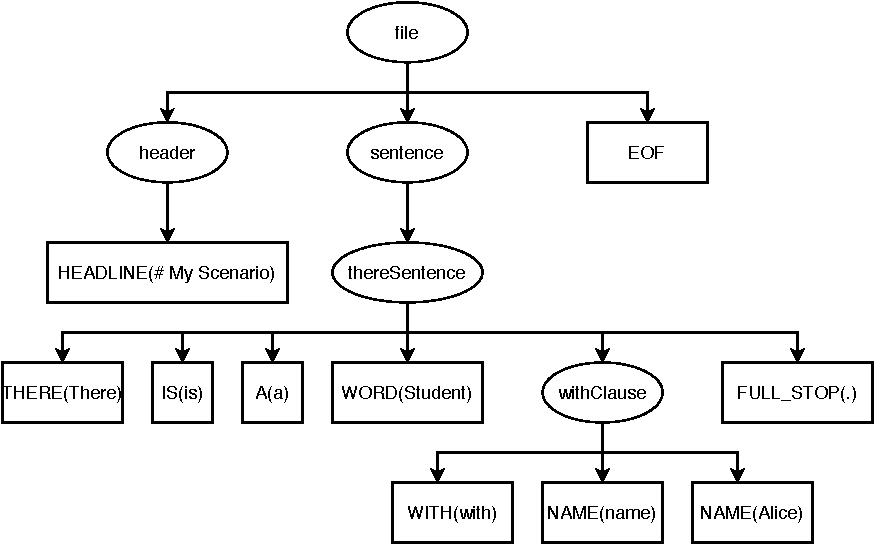
\includegraphics[width=\textwidth]{chapter/fulib-scenarios/img/parsetree.pdf}
	\caption{Syntaxbaum von Listing~\ref{lst:CompilationExample.md}}
	\label{fig:parsetree}
\end{figure}

\todo{
Warum gerade ANTLR4 so gut für die Sprachstruktur geeignet ist (Erweiterbarkeit im Vergleich zu handgeschriebenem Parser,
adaptives Parsing)~\cite{adaptive-ll-star,antlr4-reference}.
}

\subsection{AST, Analyse und Transformation}\label{subsec:data-model-gentreesrc}

\todo{
AST mit GenTreeSrc;
eigenes Projekt, kurze Erklärung.
Prä-Transformation: Gruppieren von Sätzen zu Methoden
Analyse: Variablen, Konflikte bei Attributen und Assoziationen, Programmstruktur.
Transformation: Bauen von Klassenmodell, Vereinfachung des AST in Vorbereitung auf CodeGen.
}

\subsection{Codegenerierung - Fulib}\label{subsec:codegen-fulib}

\todo{
Modellgenerierung mit Fulib.
Testgenerierung selbst.
}
